% ─────────────────────────────────────────────────────────────────────────────
\chapter{Technical Background Concepts}\label{chap:background}
% ─────────────────────────────────────────────────────────────────────────────
This chapter introduces the theoretical concepts necessary to understand the
evaluation of the operational robustness of proxy models and \gls{ai}-based
software employed in \gls{df} for the automated classification or semantic
retrieval of images. The theoretical framework is built upon the foundations
of \gls{df} and digital evidence. The chapter then examines the role of
\gls{ai} in forensic workflows, the relevance of images as digital evidence,
the principles of \gls{ml} and \gls{dl} applied to computer vision,
\textbf{\gls{advml}}, anti-forensic techniques applied to visual content, and
the role of \gls{xai} in assessing model reliability. In this chapter, these
topics are framed at a conceptual level; the rationale for their selection, the
adopted configurations, and the procedures used to apply them within the
experimental protocol are discussed in the methodology chapter.

% ─────────────────────────────────────────────────────────────────────────────
\section{Digital Forensics and Digital Evidence}
\label{sec:background_df_evidence}
% ─────────────────────────────────────────────────────────────────────────────
\gls{df} is the technical and scientific discipline concerned with the
identification, acquisition, preservation, examination, analysis, and
presentation of digital data that may be relevant in an investigative or
judicial context. It arises from the need to handle information stored or
transmitted through electronic devices according to procedures suitable for
preserving its evidentiary value. From this perspective, digital data do not
automatically acquire the status of evidence: they must be collected,
documented, and interpreted through procedures that are controllable,
repeatable, and compatible with the requirements of integrity, authenticity,
and traceability demanded by forensic investigation
\cite{casey2011digital,garfinkel2010digital,nist2006guide,iso27041}.

Digital evidence presents distinctive characteristics compared with
traditional physical evidence. It is intangible, easily replicable, often
distributed across devices, cloud services, removable media, and communication
systems, and may be altered even by apparently ordinary operations, such as
powering on a device, opening a file, or executing an application. This
fragility makes it necessary to distinguish between the mere technical
availability of data and their forensic usability. An image, a log, a message,
or a multimedia file can contribute to the reconstruction of an event only if
its investigative life cycle is documented in a way that makes it possible to
verify the operations performed and any transformations it may have undergone.

The requirements of integrity, authenticity, and traceability therefore
constitute the methodological foundation of \gls{df}. Integrity concerns the
ability to demonstrate that the analyzed data have not been modified in an
uncontrolled manner with respect to the acquired source. Authenticity refers to
the possibility of linking the evidence to a specific device, subject, system,
or operational context. Traceability, finally, requires every phase of forensic
activity to be documented through records, logs, technical notes, hash values,
and chain-of-custody procedures. These elements do not serve only an
administrative function; rather, they make it possible to verify the path that
leads from the original digital item to the information presented in an
investigative or judicial setting
\cite{iso27037,enfsi2022,swgde_guidelines,acpo_guidelines}.

From an operational perspective, the literature and technical guidelines
describe the digital forensic process as a sequence of logically distinct
phases: collection, examination, analysis, and reporting \cite{iso27043}. The collection phase
concerns the identification and acquisition of relevant digital sources, with
particular attention to preserving the state of the evidence. The examination
phase includes the extraction and organization of potentially relevant data,
for example through file system analysis, artifact recovery, indexing, and
filtering. The analysis phase consists of the technical interpretation of the
extracted data, the correlation among different sources, and the reconstruction
of relevant events or behaviors \cite{iso27042}. Finally, the reporting phase
requires clear,
verifiable, and understandable documentation of the activities performed, the
tools used, the results obtained, and the limitations encountered
\cite{reith2002examining,nist2006guide,casey2011digital,carrier2005filesystem}.


Figure~\ref{fig:df_workflow} summarizes this general workflow and places the
present thesis primarily within the \textit{examination} and \textit{analysis}
phases.

\begin{figure}[htbp]
    \centering
    \resizebox{\textwidth}{!}{%
    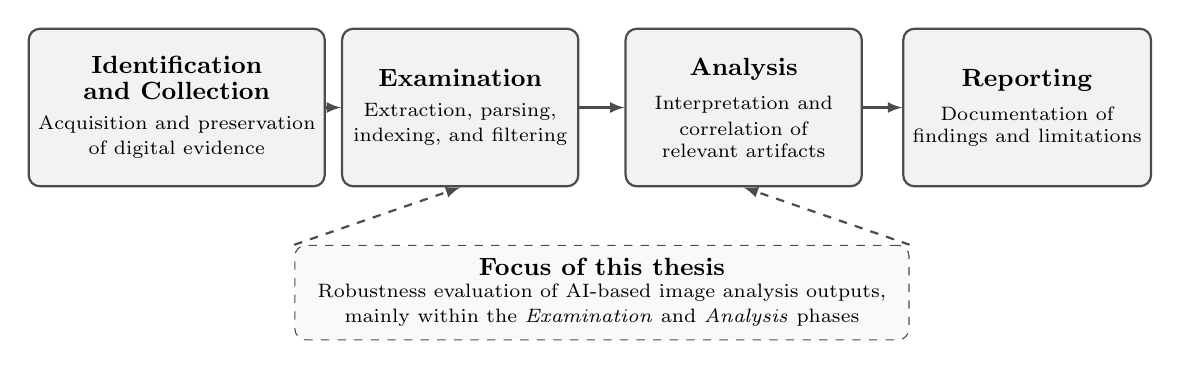
\begin{tikzpicture}[
        >=latex,
        font=\small,
        block/.style={
            rectangle,
            rounded corners,
            draw=black!70,
            thick,
            align=center,
            minimum height=2.0cm,
            minimum width=3.0cm,
            fill=gray!10
        },
        note/.style={
            rectangle,
            rounded corners,
            draw=black!70,
            dashed,
            align=center,
            minimum height=1.2cm,
            minimum width=7.8cm,
            fill=gray!5
        },
        arrow/.style={
            ->,
            thick,
            draw=black!70
        }
    ]

    \node[block] (collection) at (0,0)
    {\shortstack{
        \textbf{Identification}\\
        \textbf{and Collection}\\[1mm]
        \scriptsize Acquisition and preservation\\
        \scriptsize of digital evidence
    }};

    \node[block] (examination) at (3.6,0)
    {\shortstack{
        \textbf{Examination}\\[1mm]
        \scriptsize Extraction, parsing,\\
        \scriptsize indexing, and filtering
    }};

    \node[block] (analysis) at (7.2,0)
    {\shortstack{
        \textbf{Analysis}\\[1mm]
        \scriptsize Interpretation and\\
        \scriptsize correlation of\\
        \scriptsize relevant artifacts
    }};

    \node[block] (reporting) at (10.8,0)
    {\shortstack{
        \textbf{Reporting}\\[1mm]
        \scriptsize Documentation of\\
        \scriptsize findings and limitations
    }};

    \draw[arrow] (collection) -- (examination);
    \draw[arrow] (examination) -- (analysis);
    \draw[arrow] (analysis) -- (reporting);

    \node[note] (thesisfocus) at (5.4,-2.35)
    {\shortstack{
        \textbf{Focus of this thesis}\\
        \scriptsize Robustness evaluation of AI-based image analysis outputs,\\
        \scriptsize mainly within the \emph{Examination} and \emph{Analysis} phases
    }};

    \draw[arrow, dashed] (thesisfocus.north west) -- (examination.south);
    \draw[arrow, dashed] (thesisfocus.north east) -- (analysis.south);

    \end{tikzpicture}%
    }
    \caption{Simplified digital forensic workflow}
    \label{fig:df_workflow}
\end{figure}

% ─────────────────────────────────────────────────────────────────────────────
\subsection{Acquisition and Preservation of Digital Evidence}
\label{subsec:background_acquisition_preservation}
% ─────────────────────────────────────────────────────────────────────────────
The acquisition phase aims to make copies or extractions of digital evidence
available for examination while preserving, as far as possible, their state,
integrity, and traceability. The operational procedures depend on the nature of
the source, its state at the time of intervention, and the type of information
being sought. In general terms, a distinction can be made between the
acquisition of persistent data from storage media and the acquisition of
volatile data from active systems. In both cases, the operations performed must
be documented in a way that enables the subsequent reconstruction of the
acquisition process \cite{nist2006guide,iso27037,casey2011digital}.

In the case of storage media accessible under controlled conditions, a central
technique is physical acquisition, or \textit{bit-stream imaging}, through
which a sector-by-sector copy of the original medium is produced. Unlike a
simple logical copy of visible files, a bit-stream image may also preserve
unallocated space, \textit{slack space} areas, file system structures, and
remnants of deleted data that may be relevant to the investigation. When
technically applicable, the use of \textit{write blocking} devices makes it
possible to prevent accidental write operations on the source medium during
acquisition. The integrity of the copy is then verified through cryptographic
hash functions, such as \gls{sha256}, with the values obtained, tools used,
operators, date, and conditions of the activity documented within the chain of
custody \cite{carrier2005filesystem,iso27037,swgde_guidelines}.

Logical acquisition, by contrast, consists of extracting the data made
available by the operating system, the application, or the device under
analysis, without necessarily including the entire physical structure of the
medium. This mode may be relevant, for example, for acquiring application
content, multimedia archives, or data accessible from mobile devices and
digital services. It may allow information of interest to be obtained rapidly,
but it has limitations with respect to the completeness of the recovered data
and the availability of unallocated areas or deleted artifacts.

When the system is powered on or contains information that would be lost upon
shutdown, a \textit{live} acquisition may be necessary. This may include
volatile memory, running processes, active network connections, open sessions,
mounted encrypted volumes, or other transient elements. Live acquisition
inevitably involves interaction with the system under analysis and must
therefore be justified and documented with particular caution, specifying which
changes were introduced by the operator's activity or by the tools employed
\cite{nist2006guide,casey2011digital}.

For the purposes of this thesis, these principles are relevant because the
images subjected to automated classification must be considered digital
artifacts whose provenance, integrity, and processing history affect the
interpretation of the results. Robustness evaluation therefore does not replace
the procedures for acquiring and preserving evidence, but is situated
downstream from them, examining the reliability of automated support applied to
content that has already been acquired and organized under documented
conditions.


% ─────────────────────────────────────────────────────────────────────────────
\subsection{Examination, Analysis, and Triage of Digital Content}
\label{subsec:background_examination_analysis}
% ─────────────────────────────────────────────────────────────────────────────
Once evidence has been acquired and preserved, the \textit{examination} phase
aims to identify, extract, and organize potentially relevant artifacts. Commonly
used techniques include file system analysis, recovery of deleted files,
\textit{file carving}, metadata examination, keyword searching, content
indexing, hash-based comparison, and the extraction of artifacts generated by
operating systems or applications. These activities make it possible to reduce
the volume of raw data and isolate sets of content to be subjected to subsequent
technical and investigative assessment
\cite{carrier2005filesystem,casey2011digital,nist2006guide}.

The \textit{analysis} phase instead concerns the interpretation of the extracted
artifacts and their correlation with the investigative hypotheses. It may
include the temporal reconstruction of events through \textit{timeline
analysis}, comparison across different sources, interpretation of metadata, the
identification of relationships among files, users, or devices, and the
assessment of the investigative significance of multimedia content. In this
phase, the mere presence of a file is not sufficient: its relevance, context,
reliability, and relationship with the other available elements must be
established.

In the case of large collections of images and videos, examination and analysis
activities may be preceded or supported by triage procedures. Triage aims to
prioritize potentially relevant content without replacing the analyst's
verification. In this context, semantic search, visual grouping, and automated
classification functionalities may help highlight images compatible with
investigative categories of interest, such as the presence of a weapon.
However, the operational value of these functionalities depends on their
reliability: a false negative may reduce the likelihood that relevant content
will be examined promptly, whereas a false positive may unnecessarily increase
the review burden.

The present thesis is positioned precisely at this point in the forensic
workflow. It does not evaluate acquisition techniques or propose a method for
authenticating digital evidence, but analyzes the operational robustness of
automated classification and semantic image retrieval as forms of support for
triage and the examination of previously acquired visual content. This
distinction is methodologically essential: proper acquisition ensures
preservation of the artifact, whereas the evaluation conducted in this work
concerns the reliability of subsequent automated selection when the image is
clean, out-of-distribution, degraded, or intentionally manipulated.


% ─────────────────────────────────────────────────────────────────────────────
\section{Artificial Intelligence in Digital Forensics}
\label{sec:background_ai_digital_forensics}
% ─────────────────────────────────────────────────────────────────────────────
The integration of \gls{ai} into \gls{df} addresses the increasing
quantitative and qualitative complexity of digital investigations. The growing
volume of data acquired from personal devices, cloud infrastructures, mobile
systems, messaging applications, and multimedia archives makes an exclusively
manual analysis progressively less sustainable. In this scenario, automation
techniques, intelligent indexing, and assisted classification can support the
analyst in the preliminary selection of potentially relevant information,
reducing the operational workload and accelerating the examination and analysis
of digital evidence \cite{garfinkel2010digital,costantini2019digital}.

In forensic contexts, \gls{ai} can be employed for heterogeneous tasks,
including pattern recognition, the grouping of similar content, semantic search,
the automated classification of images and documents, anomaly detection, and
the prioritization of artifacts to be submitted to human review. These
functionalities do not replace the operator's evaluative activity, but they can
support the navigation of large datasets, especially when the evidence contains
large amounts of multimedia content or poorly structured information. The
relevance of \gls{ai} in \gls{df} should therefore be understood in terms of
investigative assistance, rather than as an automated delegation of evidentiary
decision-making \cite{costantini2019digital,faqir2023digital}.

The use of \gls{ml} and \gls{dl} models, however, introduces a discontinuity
with respect to traditional forensic tools. Many classical digital analysis
procedures rely on deterministic rules, known signatures, hashes, metadata,
keyword searches, or file system structures. Machine learning models, by
contrast, produce probabilistic outputs based on representations learned from
data. This characteristic makes it possible to process complex content, such as
images, videos, and natural language text, but it also requires closer
attention to the quality of the training data, the distribution of inputs,
model generalization, and the stability of predictions under non-ideal
conditions.

In forensic settings, this distinction is particularly relevant because the
output of an \gls{ai}-based system can influence how the analyst explores the
evidence. An incorrect classification does not necessarily determine an
autonomous evidentiary conclusion, but it may affect the priority assigned to
specific content, the visibility of relevant artifacts, or the overall
efficiency of the investigative workflow. Consequently, the reliability of an
automated module cannot be assessed solely through aggregate accuracy metrics,
but must also be considered with respect to false positives, false negatives,
distributional bias, and scenarios involving intentional manipulation.

Recent literature has shown that the use of \gls{ai}-based functionalities in
software employed for forensic analysis raises a specific validation problem:
it is not sufficient to verify that the system works correctly on ordinary
data; it is also necessary to understand its behavior in the presence of
degraded, manipulated, or out-of-distribution data
\cite{sanna2024preliminary,sanna2025pixelperfect}. This aspect is especially
important when the analysis concerns visual content, since images and videos
can be altered through compression, resizing, blurring, contrast modification,
or adversarial perturbations. Under such conditions, a system that appears
accurate on clean data may exhibit a significant reduction in its
classification capability.

For these reasons, the adoption of \gls{ai} in \gls{df} must be accompanied by
a paradigm based on human supervision, technical documentation, and experimental
evaluation of robustness. The analyst must be able to understand the role
played by the automated system, the limitations of the classification produced,
and the conditions under which the model may generate errors. From this
perspective, \gls{ai} does not represent a substitute for forensic expertise,
but rather a support tool whose usefulness depends on the possibility of
verifying its performance, stability, and reliability within the operational
context in which it is used.

The case of automated image classification constitutes a particularly
significant domain for analyzing these issues. Images may contain information
directly relevant to an investigation, but they are also subject to technical
transformations and manipulations that can modify their appearance, metadata,
or statistical characteristics. For this reason, before introducing the
principles of \gls{ml} and \gls{dl} applied to computer vision, it is necessary
to clarify the role of images as digital evidence and the meaning of their
automated classification in the context of \textit{image forensics}.


% ─────────────────────────────────────────────────────────────────────────────
\section{Image Forensics and Automated Classification}
\label{sec:background_image_forensics}
% ─────────────────────────────────────────────────────────────────────────────
Digital images represent a particularly relevant category of evidence in
contemporary forensic investigations. They may document places, objects,
persons, behaviors, tools, or circumstances that are potentially significant
for the reconstruction of an event. Unlike other digital artifacts, however,
an image combines a visual dimension that is immediately interpretable by the
human observer with a complex technical structure, consisting of pixel values,
metadata, compression parameters, information about the acquisition device, and
possible traces of subsequent processing. For this reason, forensic image
analysis requires consideration of both the depicted content and the digital
properties of the file that represents it \cite{farid2016photo,stamm2013information}.

\textit{Image forensics} focuses on the study of digital images with the aim of
assessing their origin, integrity, authenticity, and possible manipulations.
Classical techniques in this domain include, among others, metadata analysis,
the study of compression artifacts, the search for statistical inconsistencies,
the identification of resampling traces, and the examination of signals
associated with the image acquisition process. These signals include traces
produced by the photographic sensor of the acquisition device, such as the CMOS
or CCD sensor integrated into a camera or smartphone. In particular, \gls{prnu}
represents a characteristic noise component attributable to non-uniformities in
sensor response and may be used, in specific forensic analyses, to support the
attribution of an image to an acquisition device \cite{lukas2006prnu}. Such
analyses do not aim merely to establish whether an image is visually plausible,
but to verify whether the file contains technical elements compatible with a
specific origin or a specific processing history
\cite{popescu2005exposing,farid2016photo}.

In the context of the present thesis, \textit{image forensics} is considered
primarily as a conceptual framework for understanding the complexity of images
as digital evidence. The focus is not the direct detection of forgeries or
manipulations through specialized forgery detection techniques
\cite{cozzolino2017recasting}, but the evaluation of automated classification
and semantic retrieval of visual content in a forensic context. This
distinction is important: determining whether an image has been manipulated and
classifying what it represents are two different tasks, although they may
interact. A manipulation or degradation of the image may not be the primary
object of the analysis, but it may nevertheless affect the ability of an
automated tool to correctly recognize the depicted content.

Automated image classification consists of assigning an image to one or more
semantic categories on the basis of its visual content. In forensic contexts,
such categories may correspond to objects, scenes, persons, documents,
sensitive content, or elements considered relevant to an investigation. This
form of automation can support the analyst in managing large multimedia
collections, making it possible to filter, sort, or prioritize potentially
relevant images. However, automated classification must not be interpreted as
an autonomous evidentiary determination: it produces a technical indication
that requires contextualization, verification, and human supervision.

The reliability of automated classification also depends on the technical
characteristics of the image. Resolution, visual quality, illumination,
occlusions, perspective, \gls{jpeg} compression, resampling, blurring, and
color modifications can alter the digital representation of the content and
reduce the stability of predictions. Some transformations are common in normal
image production and sharing flows, for example when content is uploaded to
social platforms, forwarded through messaging applications, or saved multiple
times in compressed formats. Other transformations may instead be introduced
deliberately to degrade the image, mask details, or make automated analysis
more difficult.

This sensitivity is particularly critical in forensic contexts, because a
classification error may affect the preliminary evidence selection process. A
false negative may prevent a relevant image from being brought to the analyst's
attention, whereas a false positive may increase the review burden and generate
irrelevant investigative paths. In both cases, the problem concerns not only the
technical performance of the classifier, but also the relationship among
automation, investigative priority, and the reliability of the forensic
workflow.

Therefore, automated image classification in forensic contexts must be
evaluated by considering not only the correctness of the prediction on clean
data, but also its stability with respect to realistic conditions of
acquisition, compression, degradation, and manipulation. This aspect directly
connects \textit{image forensics} to the evaluation of the robustness of
\gls{ai}-based models. Before discussing adversarial attacks and anti-forensic
techniques, it is necessary to introduce the principles of \gls{ml} and
\gls{dl} that enable computer vision systems to learn visual representations
and produce automated classifications.


% ─────────────────────────────────────────────────────────────────────────────
\section{Machine Learning and Deep Learning for Computer Vision}
\label{sec:background_ml_dl_cv}
% ─────────────────────────────────────────────────────────────────────────────
Computer vision encompasses the set of computational methods aimed at the
automated analysis of images and videos, with the objective of extracting
structured information from visual content. In this domain, \gls{ml} and
\gls{dl} techniques have progressively replaced or complemented approaches
based on manually designed features, enabling models to learn visual
representations directly from data. In the case of image classification, the
problem consists of associating one or more semantic labels with an image on
the basis of the observable characteristics of its visual content
\cite{bishop2006pattern,gonzalez2018digital}.

Within the computer vision domain, it is useful to distinguish among related
but non-equivalent tasks. \textit{Image classification} assigns one or more
semantic labels to the entire image; \textit{object recognition} concerns the
recognition of the presence or category of an object represented in the visual
content; \textit{object detection} adds to this recognition the spatial
localization of the object, typically through regions or \textit{bounding
boxes}; finally, \textit{semantic search} enables the retrieval of images
consistent with a textual description or concept. In the present thesis, the
main experimental task is formulated as binary semantic image classification,
based on the presence or absence of firearm-related visual content of
investigative relevance, such as clearly recognizable realistic individual
firearms. Accordingly, the \texttt{weapon} class does not require the geometric
localization of the object within the image, but rather the correct
identification of the content as relevant to the forensic triage task. This
setting is consistent with studies that have applied AI-based systems to the
classification of images extracted from criminal evidence, including
operational categories such as firearms and ammunition
\cite{silva2021microservices}.

In the supervised learning paradigm, a model is trained on a set of annotated
examples, each consisting of an input and a corresponding class label. During
training, the model learns a decision function capable of associating new
inputs with one of the classes defined by the task. The objective is not to
memorize the observed examples, but to generalize correctly to unseen data.
This distinction is central in forensic contexts, because a classifier used on
real evidence may encounter images that differ from those present in the
training data in terms of quality, provenance, resolution, compression, visual
context, or semantic distribution.

The quality of generalization depends on several factors, including the
representativeness of the dataset, the consistency of the annotations, class
separability, data balance, and the model's ability to learn features that are
genuinely relevant to the task. In the absence of these conditions, a system may
achieve good performance on a controlled test set while being less reliable in
realistic scenarios. This problem is particularly relevant in forensic tasks,
where images may originate from heterogeneous sources, be degraded by
compression or sharing processes, or contain ambiguous and out-of-distribution
cases.

Traditional \gls{ml} approaches applied to image classification are often based
on a separation between feature extraction and classification. Visual features
are computed through descriptors designed or selected according to the problem,
while a classifier learns a decision rule in the feature space. Models such as
\gls{svm} have long represented an effective solution for supervised
classification problems, owing to their ability to construct robust decision
surfaces in high-dimensional spaces
\cite{cortes1995support,bishop2006pattern}. General-purpose libraries such as
scikit-learn provide standardized implementations of classical supervised-learning
algorithms and evaluation utilities, supporting reproducible experimentation
across conventional \gls{ml} workflows \cite{pedregosa2011scikit}. However, the
quality of the result depends strongly on the choice of features and on their
ability to represent image content in a discriminative manner.

\gls{dl} has profoundly changed this paradigm by introducing models capable of
automatically learning hierarchical representations of data. In \gls{cnn} architectures,
the first layers tend to capture simple visual structures, such as edges, textures, and local contrasts,
whereas deeper layers combine this information into more abstract and
semantically meaningful representations. Architectures such as ResNet have
shown the effectiveness of residual connections for training deep networks,
mitigating the degradation problem encountered during optimization and improving
the ability to learn complex visual representations \cite{he2016deep}. Later
models, such as EfficientNet, introduced more balanced scaling strategies across
depth, width, and image resolution, with the objective of improving the
relationship between performance and computational cost \cite{tan2019efficientnet}.

Alongside convolutional architectures, vision-language models capable of
learning joint representations of images and text have become increasingly
prominent in recent years. In these systems, an image is not analyzed only with
respect to predefined classes during training, but can also be associated with
textual descriptions or more general semantic concepts. Models such as
\gls{clip} have shown the possibility of learning transferable visual
representations from large-scale language supervision, opening the way to
zero-shot or text-guided classification \cite{radford2021learning}. This
approach is particularly interesting in contexts in which operational
categories do not perfectly correspond to the classes available in traditional
datasets, but it also introduces new challenges related to prompt formulation,
semantic coverage of the classes, and prediction stability.

Alongside \gls{clip}, generative vision-language models such as \gls{blip} also
make it possible to associate images with textual descriptions, introducing a
complementary perspective with respect to closed-set classification based on
predefined labels \cite{li2022blip}. In forensic contexts, such models may
support forms of automated description of visual content and contribute to the
preliminary prioritization of multimedia artifacts. However, their use requires
particular caution, because the generated description may be sensitive to image
quality, data distribution, prompt formulation, and the presence of ambiguous
or out-of-distribution content.

In the experimental protocol of the present thesis, \gls{blip} is not used as a
main proxy model. Its introduction in the background serves a contextual
function, as it helps frame the evolution of vision-language models and their
possible use in scenarios involving automated image analysis. The experimental
evaluation instead focuses on proxy models that are more directly comparable in
the binary \texttt{weapon}/\texttt{non\_weapon} task and on \gls{ai}-based
software selected for operational evaluation in a forensic context. For the
latter, analyzed in a black-box setting, the thesis does not assume any
specific internal architecture for recognition, retrieval, tagging, or object
localization, but evaluates the observable behavior of the outputs available to
the analyst, such as classifications, tags, semantic bookmarks, or
visual and semantic retrieval results, with respect to the experimental conditions
considered.


From a forensic perspective, model choice cannot be assessed exclusively as a
function of average accuracy. An automated classification system must also be
considered with respect to its behavior on heterogeneous, degraded, ambiguous,
or out-of-distribution data.

Such inputs may produce incorrect closed-set assignments or predictions
associated with high maximum predicted-class probabilities. Evaluating
\gls{ood} behavior therefore makes it possible to observe how frequently
content outside the nominal task is assigned to the known operational classes
and how the corresponding probability outputs are distributed
\cite{hendrycks2017baseline,fort2021exploring}.

These probability values remain architecture-specific and may not be
calibrated. They must therefore be interpreted as intra-model diagnostic
outputs rather than as direct measures of correctness, certainty, or forensic
reliability.

This setting motivates the introduction of a separate experimental
\gls{ood} branch, distinct from the two supervised operational classes. In the
present thesis, this branch represents borderline, anomalous, degraded,
synthetic, or otherwise out-of-task content with respect to the
\texttt{weapon}/\texttt{non\_weapon} task.

The branch is evaluated separately and is not used to train a three-class
classifier. Its inclusion also does not presuppose that the black-box software
systems implement a dedicated \gls{ood}-detection mechanism or expose an
explicit unknown state.




A further aspect concerns the probabilistic interpretation of outputs. Many
classification models produce scores or probabilities associated with classes,
but these values do not necessarily correspond to a direct measure of
evidentiary reliability. High confidence may result from spurious correlations,
dataset bias, or overfitting to the training distribution. For this reason, the
use of \gls{ml} and \gls{dl} models in a forensic workflow requires a cautious
assessment in which automated predictions are considered analytical support
rather than autonomous determinations.

Forensic computer vision must therefore confront a methodological tension: on
the one hand, \gls{dl} models make it possible to analyze large quantities of
images with performance that is often superior to traditional approaches; on
the other hand, their reliability may decrease in the presence of visual
variations, anti-forensic transformations, adversarial perturbations, or
out-of-distribution inputs. This tension justifies the need to study the
robustness of classifiers not only under clean and controlled conditions, but
also in realistic scenarios in which visual content may be degraded,
manipulated, or deliberately altered.

% ─────────────────────────────────────────────────────────────────────────────
\section{Adversarial Machine Learning}
\label{sec:background_adversarial_ml}
% ─────────────────────────────────────────────────────────────────────────────
\gls{advml} studies the behavior of machine learning systems in the presence of
inputs constructed or modified with the aim of altering their operation. Unlike
errors due to random noise, poor data quality, or generalization limits,
adversarial attacks presuppose the presence of an actor who deliberately
modifies the input in order to induce the model to produce an incorrect
prediction. In the computer vision domain, this problem is particularly
relevant because small variations in digital content may be sufficient to
change the classification produced by a model, even when the image remains
apparently similar to a human observer
\cite{szegedy2014intriguing,goodfellow2015explaining}.

An adversarial example can be described, in general terms, as an input modified
with respect to an original sample, but constructed so as to induce the
classifier to produce an incorrect label. Let \(x\) denote the original image,
\(y\) its correct class, and \(f(\cdot)\) the classifier. The attacker's
objective is to generate a perturbed version \(x'\), such that \(x'\) remains
sufficiently close to \(x\) according to a distance or perceptibility
constraint, but is classified differently by the model. In simplified form, the
problem can be expressed as the search for a perturbation \(\delta\) such that:
\[
x' = x + \delta
\quad \text{and} \quad
f(x') \neq y.
\]

The perturbation \(\delta\) is often constrained by distance metrics or
\(\ell_p\)-norm constraints, expressed as \(\|\delta\|_p \leq \epsilon\), where
\(\epsilon\) represents the maximum allowed perturbation budget and, in the most
common cases, \(p \in \{0,2,\infty\}\). These constraints make it possible to
formalize sparse attacks, limited-energy perturbations, or modifications that
are uniformly bounded across pixels, respectively, although they do not exhaust
the problem of visual perceptibility in real-world scenarios
\cite{carlini2017towards,akhtar2018threat}.

This formulation highlights the dual nature of the attack: on the one hand, the
perturbation must be limited; on the other hand, it must be sufficiently
effective to change the system's decision.

Figure~\ref{fig:adv_example} conceptually represents this mechanism in the
context of an evasion attack.

\begin{figure}[htbp]
    \centering
    \resizebox{\textwidth}{!}{%
        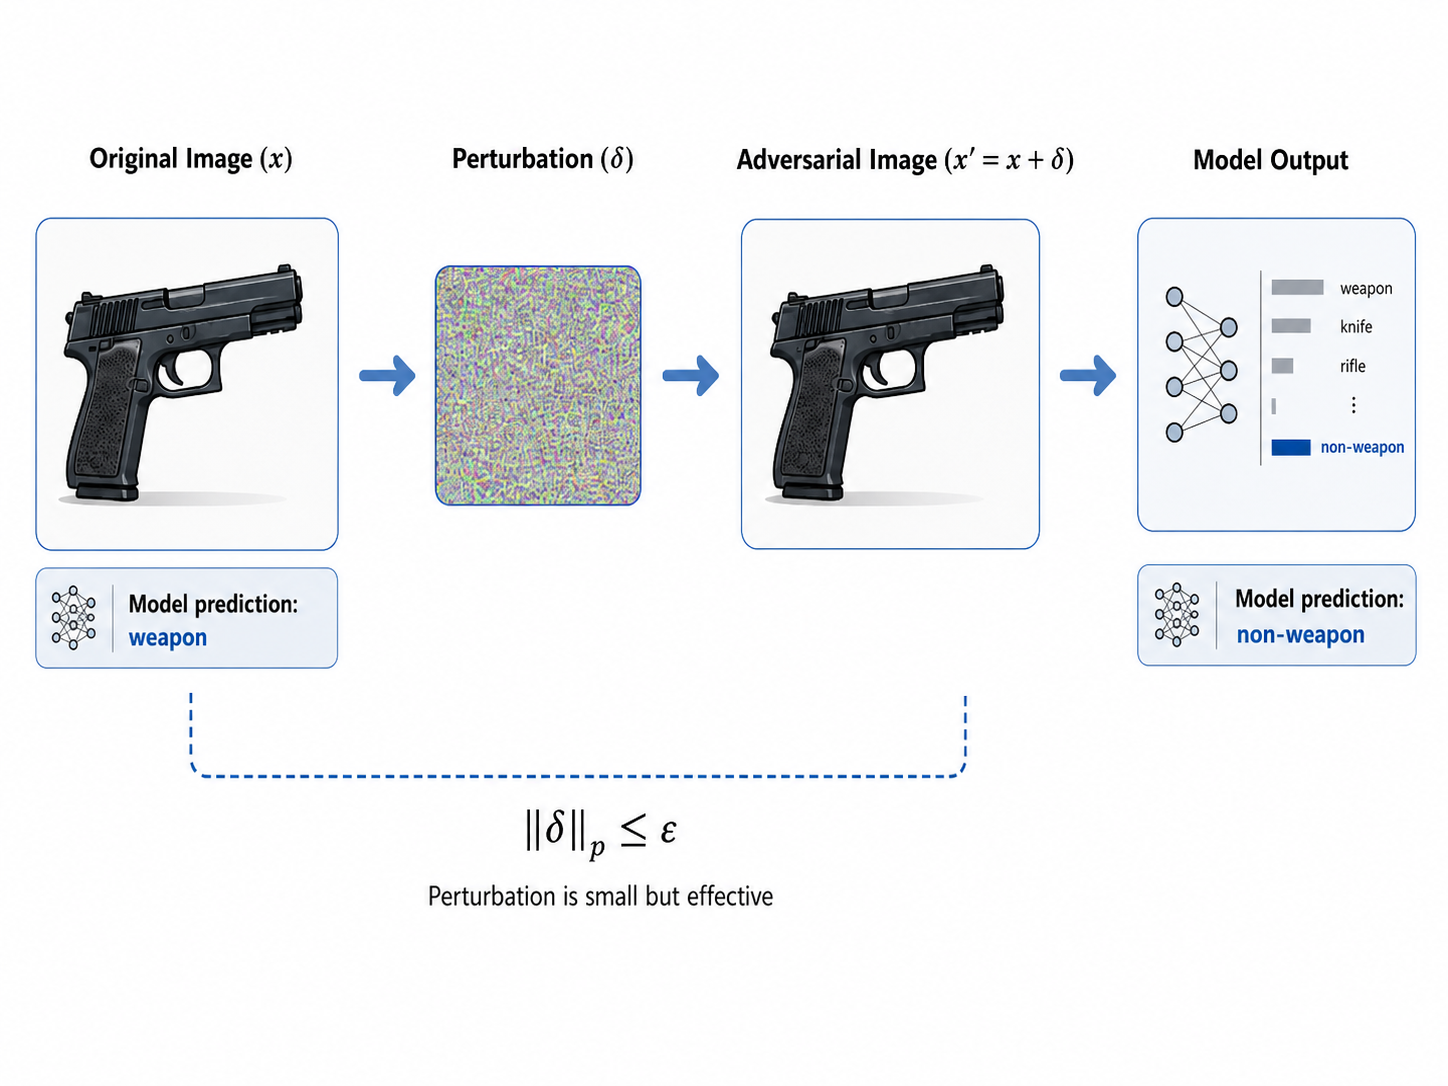
\includegraphics{images/adversarial_example_logic}
    }
\caption[Conceptual representation of an adversarial evasion attack]{Conceptual representation of an adversarial evasion attack. A bounded perturbation \(\delta\) is added to the original input \(x\) to obtain an adversarial image \(x'\), which induces a wrong classifier prediction while preserving visual coherence for a human analyst}
    \label{fig:adv_example}
\end{figure}

Adversarial attacks can be classified according to several criteria. A first
distinction concerns the phase of the model life cycle in which the attack is
conducted. Poisoning attacks occur during the training phase, by altering the
data or labels with the aim of compromising the resulting model. Evasion
attacks, by contrast, occur at inference time and consist of manipulating the
inputs submitted to an already trained model
\cite{biggio2018wild,papernot2016limitations}. In the context of automated
image classification in forensic settings, the main focus is on evasion
attacks, because the most relevant scenario is one in which images already
present on a device, in an archive, or within digital evidence are altered to
reduce the likelihood of being correctly identified by an automated tool.

A second distinction concerns the level of knowledge available to the attacker.
In white-box scenarios, the attacker has complete or extensive information
about the model, including its architecture, parameters, loss function, and
gradients. In these cases, the perturbation can be optimized directly with
respect to the internal behavior of the classifier. In black-box scenarios, by
contrast, the attacker does not know the details of the model and may rely only
on observable outputs, repeated queries, surrogate models, or the
transferability of adversarial examples across different classifiers
\cite{papernot2016limitations,carlini2017towards,yuan2019adversarial}. This
distinction is particularly important in the present thesis, because the
commercial software selected for operational evaluation is observed in a
black-box setting and does not allow assumptions about access to the parameters
or internal logic of any AI-based components.

A further distinction concerns the objective of the attack. In untargeted
attacks, the intent is simply to induce the model to produce a class different
from the correct one. In targeted attacks, by contrast, the objective is to
push the classifier toward a specific class chosen by the attacker. In the case
of forensic images, an untargeted attack may be sufficient to reduce the
ability of the tool to retrieve relevant content, whereas a targeted attack
could aim to make sensitive content appear as if it belonged to an innocuous
category. However, in an evidentiary context, even less controlled forms of
error may have significant operational consequences, because they affect the
selection, prioritization, and review of digital evidence.

The literature has proposed numerous techniques for generating adversarial
examples, differentiated by perturbation constraint, computational cost,
required knowledge, and transferability. Gradient-based methods, such as
\gls{fgsm}, exploit the information provided by the loss function to identify
an effective perturbation direction \cite{goodfellow2015explaining}. Other
approaches aim to produce more optimized, sparser, or more localized
perturbations, reducing the number of modified pixels or approximating minimal
perturbations capable of crossing the classifier's decision boundary
\cite{carlini2017towards,su2019onepixel,moosavi2016deepfool,zhang2024superdeepfool}.
In this chapter, these techniques are framed at a conceptual level; the
rationale for their selection, the adopted configurations, and the procedures
used to apply them within the experimental protocol are discussed in the
methodology chapter.

In forensic contexts, the adversarial problem does not concern only the
abstract vulnerability of models, but also their operational reliability within
an investigative process. If an \gls{ai}-based system is used to filter or
classify large quantities of images, a perturbation capable of altering its
prediction may reduce the likelihood that relevant content will be promptly
brought to the analyst's attention. The risk does not necessarily consist in
the automated production of an incorrect judicial decision, but rather in the
possibility that automation may modify the path of discovery, prioritization,
and interpretation of evidence. For this reason, adversarial robustness must be
considered a component of the broader technical-forensic reliability of the
system.

% ─────────────────────────────────────────────────────────────────────────────
\subsection{Threat Model and Attacker Assumptions}
\label{subsec:background_threat_model}
% ─────────────────────────────────────────────────────────────────────────────
The threat model defines the assumptions concerning the attacker's capabilities,
objectives, and constraints. In \gls{advml}, it is necessary to rigorously
delimit the attack scenario and to avoid robustness evaluations that lack an
operational context. Without an explicit threat model, the result of an
adversarial test risks being difficult to interpret, because it is not clear
which type of adversary the system is able to tolerate and which conditions are
instead excluded from the analysis
\cite{carlini2017towards,yuan2019adversarial}.

In the context of automated image classification in forensic settings, the
attacker can be modeled as an actor interested in reducing the likelihood that
specific content will be correctly identified by an automated tool. The main
objective is not necessarily to compromise the entire forensic workflow, but to
alter the classifier's response on specific visual inputs. In operational
terms, this may translate into the attempt to transform a relevant image into
one classified as non-relevant, ambiguous, or belonging to a category different
from the expected one. This scenario is consistent with an evasion attack,
because the manipulation affects the analyzed input rather than the model
training phase.

The attacker's capabilities may vary depending on the level of access to the
target system. In a white-box scenario, the attacker has complete or extensive
information about the model, including its architecture, parameters, loss
function, and gradients, and can therefore construct perturbations directly
optimized with respect to the classifier. In a black-box scenario, by contrast,
the attacker does not have access to the internal logic of the target system
and may rely on observable outputs, surrogate models, or the transferability of
adversarial examples. In the protocol of the present thesis, white-box access is
relevant for the controlled evaluation of proxy models when required by the
specific attack technique, whereas the selected commercial software is observed
in a black-box setting, since its internal classification logic is not
available. This distinction affects the type of attack that can be applied, the
required computational cost, and the operational plausibility of the threat.

The threat model must also specify the constraints imposed on the perturbation.
In the image domain, the modification may be limited in terms of numerical
magnitude, perceptual distance, number of altered pixels, affected image area,
or admissible transformations. In forensic contexts, these constraints acquire
a specific meaning: an excessively visible manipulation may be detected by the
human analyst or by integrity-control procedures, whereas a subtler
modification may preserve the visual plausibility of the image while still
altering the model prediction. The notion of imperceptibility must therefore be
treated with caution, because human perception, file quality, and the
investigative relevance of visual details do not necessarily coincide with a
simple mathematical distance metric.

A further aspect concerns the attacker's knowledge of the forensic domain. In
realistic scenarios, the attacker may not know the specific tool used by the
analyst, but may be aware that images and multimedia content are often subjected
to automated classification. This partial knowledge may be sufficient to
motivate transformations aimed at reducing the automatic recognizability of the
content, especially when such transformations do not clearly compromise the
general readability of the image. Therefore, the threat model must consider not
only a highly informed attacker, but also scenarios in which the adversary
operates with limited knowledge of the model and exploits generic or
transferable transformations. The operational relevance of this assumption is
consistent with the literature on adversarial examples in physical or otherwise
non-purely digital scenarios, which shows that some perturbations may retain
effectiveness even outside strictly controlled experimental conditions
\cite{kurakin2017physical}.

The threat model outlined in this subsection specifically concerns adversarial
attacks, namely perturbations constructed with the objective of altering the
classifier's response. The anti-forensic transformations discussed in the
following section instead constitute a conceptually distinct category: they may
be applied even in the absence of knowledge about the model or about any
automated classification system, and they are more generally aimed at
concealing, degrading, or making digital evidence less informative. In the
experimental protocol of the present thesis, the two categories are therefore
evaluated separately: on the one hand, adversarial perturbations oriented toward
inducing errors in the model decision; on the other hand, realistic
anti-forensic transformations not optimized with respect to the classifier,
applied to observe the stability of automated support in the presence of
plausible image manipulations. Their relationship is considered only at the
level of operational effects, since both may reduce the likelihood that
content of investigative relevance will be correctly flagged or prioritized for
subsequent analyst review.

Table~\ref{tab:threat_model} summarizes the main dimensions of the adversarial
threat model adopted in the experimental evaluation, distinguishing between the
theoretical formulation of the attacks and the operational-forensic focus of
the present thesis.

\begin{table}[htbp]
    \centering
    \small
    \renewcommand{\arraystretch}{1.25}
    \begin{tabular}{@{}p{0.24\textwidth}p{0.34\textwidth}p{0.34\textwidth}@{}}
        \toprule
        \textbf{Dimension} & \textbf{Theoretical scenarios} & \textbf{Thesis operational focus} \\
        \midrule
        \textbf{Attack phase} &
        Poisoning vs evasion &
        \textbf{Evasion}, since the manipulation affects already acquired or analyzed images at inference time. \\
        \textbf{Adversary knowledge} &
        White-box vs black-box &
        \textbf{White-box for controlled proxy-model evaluation, where required by the attack; black-box for commercial software}, whose internal \gls{ai}-based image-analysis logic is not available. \\
        \textbf{Attack objective} &
        Targeted vs untargeted &
        \textbf{Untargeted}, with emphasis on performance degradation, missed detection, and reduced classification reliability. \\
        \bottomrule
    \end{tabular}
    \caption{Adversarial threat model dimensions considered in the experimental robustness evaluation}
    \label{tab:threat_model}
\end{table}


\subsection{Adversarial and Adversarial-Style Perturbation Families}
\label{subsec:background_attack_families}

Within the general framework of \gls{advml}, this thesis considers a set of
perturbations included in the adversarial evaluation, comprising both attacks
constructed with respect to model behavior and a model-agnostic
\textit{adversarial-style} transformation. The choice is not intended to cover
the entire landscape of existing techniques exhaustively, but rather to include
perturbations that are heterogeneous in terms of computational cost, level of
knowledge required about the model architecture, alteration constraint, and
operational plausibility. In particular, gradient-based, sparse, iterative, and
model-agnostic perturbations are considered, in order to observe the behavior
of AI-based systems with respect to manipulations characterized by different
properties.

The \textbf{\acrfull{fgsm}} represents a simple and efficient adversarial
baseline. Given a classifier \(f\), a loss function \(\mathcal{L}\), an image
\(x\), and the corresponding correct label \(y\), the attack generates a
perturbed image by moving in the direction of the sign of the gradient of the
loss with respect to the input:
\[
x' = x + \epsilon \cdot \operatorname{sign}
\left(\nabla_x \mathcal{L}(f(x), y)\right).
\]
The parameter \(\epsilon\) controls the maximum magnitude of the perturbation.
In the experimental context of the thesis, \gls{fgsm} is relevant because it
makes it possible to rapidly evaluate the classifier's sensitivity to a
single-step white-box perturbation constructed directly with respect to the
model's loss function \cite{goodfellow2015explaining}.

The \textbf{\gls{onepixel}} instead represents a family of sparse and black-box
attacks, in which the perturbation is constrained to modify a very limited
number of pixels. In general form, the objective is to find a version \(x'\) of
the image such that:
\[
f(x') \neq f(x)
\quad \text{with} \quad
\|x - x'\|_0 \leq k,
\]
where \(k\) denotes the maximum number of pixels that can be modified. In the
extreme case of the \gls{onepixel}, \(k=1\). The attack is relevant because it
shows how highly localized variations can alter the decision of a neural
network, even without direct access to the model gradients
\cite{su2019onepixel}.

\textbf{\gls{sigmazero}} belongs to the family of attacks oriented toward
sparsity and the \(L_0\) norm. Unlike attacks that limit the global magnitude
of the perturbation through \(L_2\) or \(L_\infty\) norms, \(L_0\) attacks aim
to reduce the number of modified input components. The objective can be
expressed as the search for an adversarial image \(x^{adv}\) such that:
\[
f(x^{adv}) \neq f(x)
\quad \text{while minimizing} \quad
\|x - x^{adv}\|_0.
\]
This setting is particularly significant in forensic contexts because sparse
perturbations may be difficult to identify through ordinary visual inspection
and may not visibly degrade the perceptual quality of the image
\cite{zhao2024sigmazero}.

\textbf{\gls{superdeepfool}} is regarded as an iterative attack inspired by
the DeepFool family. The general idea behind DeepFool is to iteratively
estimate a perturbation capable of crossing the classifier's decision boundary,
seeking a modification of limited magnitude that is sufficient to change the
model's prediction. In abstract form, the objective is to find a perturbation
\(\delta\) such that:
\[
x' = x + \delta
\quad \text{and} \quad
f(x') \neq f(x),
\]
with \(\delta\) constructed through successive updates guided by the local
geometry of the decision function. In the context of the thesis, this family of
attacks is relevant because it represents iterative perturbations that are more
structured than a single-step attack such as \gls{fgsm}, without attributing to
the technique any general ability to overcome every possible defense or form of
pre-processing \cite{moosavi2016deepfool,zhang2024superdeepfool}. This caution
is consistent with the literature showing that some defenses may produce only
apparent robustness, for example through gradient masking or obfuscated
gradients, without ensuring genuine resistance to adaptive attacks
\cite{athalye2018obfuscated}.

A further attack frequently used in the evaluation of adversarial robustness is
\gls{pgd}, which extends the idea of gradient-based attacks through iterative
updates constrained within a perturbation neighborhood and has been widely used
as a reference for formulating adversarial robustness as a model security
problem \cite{madry2018towards}. In the present thesis, however, \gls{pgd} is
not included in the main experimental protocol. This choice stems from the need
to keep the workflow computationally sustainable and focused on operational
robustness in forensic contexts, using \gls{superdeepfool} and \gls{sigmazero}
as representatives of iterative and sparse perturbations, respectively, in line
with the objectives of the experimental protocol.

Alongside attacks constructed with respect to model behavior, the thesis also
considers a model-agnostic perturbation based on shifting color channels.
\textbf{\gls{colorshift}} globally modifies the chromatic representation of the
image, for example through offsets or multiplicative factors applied to the
\(R\), \(G\), and \(B\) channels. It represents an intermediate case with
respect to the classical distinction between model-dependent adversarial attacks
and anti-forensic transformations. In this thesis, it is treated as a
model-agnostic \textit{adversarial-style} perturbation: it does not use
gradient information and does not directly optimize a model loss function, but
it is applied with the experimental purpose of evaluating the effect of
semantically conservative alterations on automated classification. For this
reason, although it shares some visual characteristics with realistic image
transformations, it is kept within the experimental group of adversarial
perturbations, explicitly qualifying it as a model-agnostic
\textit{adversarial-style} transformation and not as an attack optimized with
respect to the model.

Table~\ref{tab:background_attack_families} summarizes the adversarial and
\textit{adversarial-style} perturbations considered in the experimental
protocol.

\begin{table}[htbp]
    \centering
    \small
    \renewcommand{\arraystretch}{1.25}
    \begin{tabularx}{\textwidth}{@{}l l X@{}}
        \toprule
        \textbf{Technique} & \textbf{Family} & \textbf{Methodological relevance} \\
        \midrule
        \gls{fgsm} &
        Gradient-based, single-step &
        Efficient white-box baseline for evaluating the model's sensitivity
        to the gradient of the loss function. \\
        \gls{onepixel} &
        Sparse, black-box &
        Highly localized perturbation, useful for evaluating vulnerability to
        minimal modifications in the pixel domain. \\
        \gls{sigmazero} &
        Sparse, \(L_0\)-oriented &
        Attack oriented toward minimizing the number of modified pixels,
        relevant to scenarios in which the perturbation must remain localized. \\
        \gls{superdeepfool} &
        Iterative boundary-based &
        Iterative attack inspired by DeepFool, useful for exploring decision
        stability with respect to crossing the decision boundary. \\
        \gls{colorshift} &
        Adversarial-style, model-agnostic &
        Semantically conservative global chromatic alteration, not optimized
        with respect to the model, included among adversarial perturbations to
        evaluate the effect of controlled color variations on automated
        outputs. \\
        \bottomrule
    \end{tabularx}
    \caption{Adversarial and adversarial-style perturbations considered in the experimental protocol}
    \label{tab:background_attack_families}
\end{table}



% ─────────────────────────────────────────────────────────────────────────────
\section{Anti-Forensic Techniques Applied to Digital Images}
\label{sec:background_antiforensics_images}
% ─────────────────────────────────────────────────────────────────────────────
Anti-forensic techniques comprise the set of strategies aimed at hindering,
degrading, or making the forensic analysis of digital content less reliable. In
the image domain, such techniques may affect both the visual properties of the
content and the statistical and structural characteristics of the file, with
the objective of reducing the possibility of reconstructing the image history,
detecting manipulations, identifying acquisition traces, or correctly
classifying the depicted content. In general terms, anti-forensics does not
necessarily coincide with the explicit forgery of an image, but also includes
transformations capable of altering or masking information relevant to
technical analysis \cite{stamm2010anti,yaacoub2021digital}.

In the context of \textit{image forensics}, many analyses rely on the presence
of statistical and structural traces associated with the formation or
subsequent processing of the image file. Such traces may include compression
artifacts, patterns introduced by resampling operations, inconsistencies among
image regions, and signals attributable to the acquisition device, such as the
\gls{prnu} of the photographic sensor. Anti-forensic transformations may aim to
reduce the visibility or reliability of these indicators, making it more
difficult to distinguish between original, degraded, or manipulated content.
For example, \gls{jpeg} recompression may modify the artifacts produced by
previous saving operations; resampling may alter the spatial correlations
introduced by resizing operations; histogram or contrast modifications may
change the distribution of image intensity values
\cite{popescu2005exposing,farid2016photo,lukas2006prnu}.

In the present thesis, these techniques are discussed to frame the domain of
\textit{image forensics} and the possible manipulations of visual evidence; the
experimental evaluation does not concern source attribution through
\gls{prnu}, but rather the stability of semantic image classification with
respect to selected transformations applied in a controlled manner.

A first family of transformations concerns compression and recompression. The
\gls{jpeg} format, widely used in digital devices and sharing platforms,
applies lossy compression that modifies the frequency components of the image
and introduces artifacts depending on the selected quality level. From a
forensic perspective, such artifacts may be informative, but they may also
interfere with subsequent analyses. Intentional recompression may attenuate or
overwrite previous traces, reduce perceptual quality, or modify statistical
characteristics exploited by automated tools. For this reason, compression is
not only a normal technical step in image management, but may also become a
relevant transformation from an anti-forensic standpoint
\cite{stamm2010anti,stamm2013information}.

A second category includes geometric and resampling operations, such as
resizing, cropping, rotation, and resampling. These transformations may be
common in ordinary image production and sharing workflows, but they may also be
used to modify the scale of objects, remove relevant regions, alter scene
composition, or introduce statistical patterns different from the original
ones. Resampling, in particular, may leave traces detectable through forensic
analysis, but it may also be combined with additional transformations to make
its identification more difficult \cite{popescu2005exposing,farid2016photo}.

Additional anti-forensic transformations concern controlled visual degradation.
Blurring, noise, resolution reduction, sharpness alteration, and color
modifications may decrease the readability of relevant details without
necessarily making the image unusable for a human observer. In an
\gls{ai}-assisted forensic workflow, these transformations are particularly
important because they may modify the visual features used by classifiers. An
object that remains recognizable to the analyst may become less discriminative
for the model, especially if the transformation alters edges, textures, local
contrasts, or spatial relationships among the components of the scene.

Alongside visible or statistically detectable transformations, a further
category of techniques attributable to the anti-forensic domain concerns
steganography, namely the concealment of information within digital content. In
the case of images, additional data may be embedded by altering poorly
perceptible portions of the representation, such as the least significant bits
of pixel values. Although steganography has different purposes from visual
degradation or recompression, it is relevant within the framework of
\textit{image forensics} because it may introduce hidden content, modify the
statistical properties of the file, and require specialized analyses to
distinguish between an apparently ordinary image and an image used as a
concealment vector \cite{stamm2013information,yaacoub2021digital}.

In the present work, steganography is mentioned as a broader component of the
anti-forensic domain, whereas the experimental evaluation focuses on visual and
statistical transformations directly relevant to the robustness of automated
classification.

It is important to distinguish anti-forensic techniques from the adversarial
attacks discussed in the previous section. Adversarial attacks are generally
designed with respect to the behavior of a model and aim to induce an incorrect
prediction through optimized perturbations. Anti-forensic transformations, by
contrast, may be model-independent and more generally oriented toward
degrading, masking, or altering digital evidence. This distinction does not
imply an absolute separation: an anti-forensic transformation may produce
adversarial effects on a classifier, just as an adversarial perturbation may
have anti-forensic consequences when it reduces the investigative usefulness of
an image. However, from a methodological standpoint, the two categories must be
kept distinct because they presuppose different attacker capabilities,
objectives, and assumptions.

In the case of automated image classification, anti-forensic techniques are
relevant because they may affect the operational robustness of \gls{ai}-based
systems even in the absence of an attack optimized against the model. A
recompressed, resized, blurred, or contrast-altered image may represent a
realistic input, compatible with ordinary acquisition, storage, or sharing
processes. However, the same transformations may be intentionally exploited to
reduce the likelihood that content will be correctly classified. The difficulty
therefore lies in distinguishing between ordinary degradations within the
digital image life cycle and transformations applied with the purpose of
concealment or reduction of analytical effectiveness.

From a forensic perspective, this ambiguity requires cautious evaluation. Not
every compressed, resized, or degraded image can be considered the result of
anti-forensic conduct; on the contrary, many transformations are ordinary
consequences of the use of mobile devices, social networks, messaging
applications, and storage systems. However, when the objective is to evaluate
the reliability of automated tools, it is necessary to include such
transformations within the space of realistic scenarios. The robustness of a
forensic classifier depends not only on its accuracy on clean images, but also
on its ability to maintain stable behavior in the presence of plausible,
intentional, or accidental degradations.

From this perspective, anti-forensic techniques applied to digital images
constitute a bridge between traditional \textit{image forensics} and the
evaluation of the robustness of computer vision models. They highlight that an
image is not a static and neutral input, but a digital artifact subject to
technical transformations that may affect both its human interpretability and
its automated processing. For this reason, the evaluation of \gls{ai}-based
models and software employed in the context of \gls{df} must consider not only
formally defined adversarial attacks, but also manipulations and degradations
compatible with realistic operational scenarios.



% ─────────────────────────────────────────────────────────────────────────────
\subsection{Image-Level Anti-Forensic Transformation Families}
\label{subsec:background_antiforensic_transformations}
% ─────────────────────────────────────────────────────────────────────────────
In the context of the present thesis, anti-forensic transformations are
considered as realistic manipulations of the image artifact, not necessarily
optimized with respect to a specific classifier. They act on the visual,
statistical, or geometric properties of the file and may derive both from
ordinary acquisition, saving, and sharing processes and from intentional
applications aimed at reducing the effectiveness of automated analysis. For
this reason, such transformations constitute a bridge between traditional
\textit{image forensics} and the evaluation of the operational robustness of
\gls{ai}-based systems.

The \textbf{\gls{jpegrecompression}} transformation consists of saving an image
again using lossy compression. Since the \gls{jpeg} format operates on the
frequency components of the image and introduces artifacts depending on the
selected quality level, recompression may modify or overwrite previous traces,
alter local statistics, and degrade visual details relevant to classifiers.
From a forensic perspective, this transformation is relevant because it may
interfere both with analyses based on compression artifacts and with
\gls{ai}-based models that are sensitive to textures, edges, and local patterns
\cite{stamm2010anti,stamm2013information}.

The \textbf{\gls{resampleresize}} transformation modifies the resolution and
spatial grid of the image. Let \(x\) denote the original image. A resizing
transformation can be modeled as:
\[
x' = \mathcal{R}(x; s, \mathcal{I}),
\]
where \(s\) is the scaling factor and \(\mathcal{I}\) represents the
interpolation method. When an image is reduced and subsequently restored to its
original size, part of the spatial information is lost and replaced by
interpolated values. This process may alter pixel correlations, geometric
traces, and local patterns used by both forensic tools and classification
models \cite{popescu2005exposing,farid2016photo}.

The \textbf{\gls{gaussianblur}} transformation introduces controlled blurring
through convolution with a Gaussian kernel. In simplified form, the operation
can be described as:
\[
x' = x * G_{\sigma},
\]
where \(G_{\sigma}\) is a two-dimensional Gaussian function and \(*\) denotes
convolution. This transformation attenuates high frequencies, reduces edge
sharpness, and may decrease the discriminative value of local details. In the
context of automated classification, blur is relevant because many \gls{cnn}
models learn features in the first convolutional layers that are strongly
related to edges, textures, and local intensity variations.

The \textbf{\gls{histogrammodification}} transformation acts on the distribution
of image intensity values. In the case of \textit{histogram equalization}, the
objective is to remap intensity levels using the cumulative distribution
function, according to a transformation of the following form:
\[
x'_i = \left\lfloor (L-1)\cdot \operatorname{CDF}(x_i) \right\rfloor,
\]
where \(L\) denotes the number of intensity levels and \(\operatorname{CDF}\) is
the normalized cumulative distribution. This transformation may improve
perceived contrast, but it may also modify global and local statistics used by
image forensics tools and automated classifiers \cite{barni2018cf}.

The \textbf{\gls{contraststretching}} transformation applies a linear
normalization of the dynamic range. Let \(I_{\min}\) and \(I_{\max}\) denote two
intensity bounds, possibly computed through percentiles to reduce the influence
of outliers. The transformation can be expressed as:
\[
x'_i =
\begin{cases}
0, & \text{if } x_i \leq I_{\min}, \\
255, & \text{if } x_i \geq I_{\max}, \\
\dfrac{x_i - I_{\min}}{I_{\max} - I_{\min}} \cdot 255, & \text{otherwise}.
\end{cases}
\]
This operation modifies the global contrast of the image and may alter the
response of models with respect to dark regions, overexposed areas, or regions
with low tonal separation.

Table~\ref{tab:background_antiforensic_transformations} summarizes the
anti-forensic transformations considered in the experimental protocol.

\begin{table}[htbp]
    \centering
    \small
    \renewcommand{\arraystretch}{1.25}
    \begin{tabularx}{\textwidth}{@{}lX@{}}
        \toprule
        \textbf{Transformation} & \textbf{Methodological relevance} \\
        \midrule
        \gls{jpegrecompression} &
        Modifies compression artifacts, frequency components, and local image
        details. \\
        \gls{resampleresize} &
        Alters the spatial grid, introduces interpolation, and may degrade
        geometric correlations and local patterns. \\
        \gls{gaussianblur} &
        Attenuates high frequencies, edges, and textures, reducing the
        discriminative value of potentially relevant details. \\
        \gls{histogrammodification} &
        Remaps the distribution of intensity levels, modifying global and local
        image statistics. \\
        \gls{contraststretching} &
        Normalizes the dynamic range and alters global contrast, with possible
        effects on the features learned by classifiers. \\
        \bottomrule
    \end{tabularx}
    \caption{Anti-forensic transformations considered in the experimental protocol}
    \label{tab:background_antiforensic_transformations}
\end{table}

Table~\ref{tab:adv_vs_antiforensics} summarizes the conceptual distinction
between \textit{adversarial attacks} and \textit{anti-forensic transformations}
in the context of automated image classification.

\begin{table}[htbp]
    \centering
    \small
    \renewcommand{\arraystretch}{1.25}
    \begin{tabular}{@{}p{0.22\textwidth}p{0.34\textwidth}p{0.34\textwidth}@{}}
        \toprule
        \textbf{Dimension} & \textbf{Adversarial attacks} & \textbf{Anti-forensic transformations} \\
        \midrule
        \textbf{Primary target} &
        Decision function of the \gls{ai}-based model. &
        Visual, statistical, or structural properties of the digital image file. \\
        \textbf{Nature} &
        Perturbations designed to alter the model prediction. &
        Manipulations or degradations such as \gls{jpeg} recompression, resizing, blur, or contrast modification. \\
        \textbf{Model dependency} &
        Usually direct or surrogate-based, especially in white-box or transfer-based settings. &
        Usually low or indirect, since the transformation can often be applied without knowing the classifier. \\
        \textbf{Visibility} &
        Often designed to be imperceptible, sparse, or localized. &
        Often compatible with visible degradations or ordinary image processing operations. \\
        \textbf{Forensic relevance} &
        May affect automated evidence selection by inducing false positives or false negatives. &
        May alter the evidentiary quality of the image and reduce the reliability of automated analysis. \\
        \bottomrule
    \end{tabular}
    \caption{Comparison between adversarial attacks and anti-forensic transformations in the context of automated image classification}
    \label{tab:adv_vs_antiforensics}
\end{table}

% ─────────────────────────────────────────────────────────────────────────────
\section{Explainability, Robustness, and Model Reliability}
\label{sec:background_xai_robustness}
% ─────────────────────────────────────────────────────────────────────────────

The evaluation of an \gls{ai}-based model cannot be reduced exclusively to the
measurement of its average accuracy. In a forensic context, the usefulness of an
automated system also depends on the stability of its predictions, its ability
to handle degraded or out-of-distribution inputs, the transparency of the
information provided to the analyst, and the possibility of documenting, in a
verifiable manner, the role played by the model within the investigative
workflow. Accuracy, robustness, interpretability, and reliability are therefore
complementary dimensions that must be considered jointly when an automated
classification system is used to support the analysis of digital evidence
\cite{Adadi2018,Doshi-Velez2017}.

Robustness can be defined, in general terms, as the ability of a model to
maintain stable and coherent behavior in the presence of input variations. Such
variations may be accidental, such as noise, compression, low resolution, or
non-ideal acquisition conditions, or intentional, such as adversarial
perturbations and anti-forensic transformations. In the computer vision domain,
robustness does not concern only resistance to small numerical perturbations,
but also the classifier's ability to handle realistic changes in the visual
properties of the image, the data distribution, and the quality of the analyzed
content \cite{hendrycks2019benchmarking,ford2019adversarial}.

Reliability is a broader concept than robustness. A model may be robust with
respect to a specific family of perturbations, but not necessarily reliable in a
forensic sense. Reliability requires the system to produce results that are
sufficiently stable, verifiably documented, and interpretable with respect to the
context of use. In particular, a classifier employed in a \gls{df} workflow must
be evaluated with respect to its ability to support the analyst without
replacing human judgment, to signal uncertainty or ambiguous cases, to avoid
overestimating its own confidence, and to maintain coherent performance even on
data different from those observed during training. This distinction is
essential because an output that is formally correct on average may still be
unreliable if it is not stable, verifiable, or adequately contextualized.

The role of \gls{xai} is situated within this framework. Explainability
techniques aim to provide tools for making model behavior more understandable,
especially when models operate as complex or partially opaque systems. In
computer vision, these techniques may include saliency maps, attribution
methods, visualizations of the image regions that most influence the prediction,
and local explanations of classifier behavior. Well-known examples include
model-agnostic approaches, such as LIME and SHAP, and attribution or visual
localization techniques, such as \gls{ig} and class activation mapping
\cite{Ribeiro2016,Lundberg2017,Sundararajan2017,Zhou2016}.

These approaches are not methodologically equivalent. Gradient-based
techniques, such as \gls{ig}, require access to the model and to the gradient of
the prediction with respect to the input, and are therefore applicable to the
controllable proxy models considered in the present thesis. Model-agnostic
approaches, such as LIME or some formulations of SHAP, can instead operate
through input-output queries, but their application to commercial software
evaluated in a \textit{black-box} setting depends on the availability of
adequate outputs, queryable interfaces, and reproducible experimental
conditions. For this reason, the operational choice of the explainability
technique used in the protocol is described in Chapter~\ref{chap:methodology}.

In the case of commercial black-box software, outputs such as tags,
classifications, retrieval results, or semantic bookmarks must therefore be
interpreted as observable operational signals rather than as local explanations
of the internal decision-making process. They can be normalized and evaluated
against the experimental ground truth, but they do not make it possible to
directly infer which features, image regions, or internal representations
determined the system's decision.

The use of \gls{xai} in forensic contexts must nevertheless be interpreted with
caution. A visual explanation does not constitute autonomous proof of the
correctness of the model, nor does it guarantee that the classifier has learned
concepts that are semantically coherent with human reasoning. Saliency maps,
for example, may indicate image regions relevant to the prediction, but they do
not necessarily demonstrate that the model recognized the object of interest in
the expected way. Moreover, explanations generated by different methods may
diverge from one another, and their stability may be influenced by input
perturbations or model variations \cite{Adadi2018,Carvalho2019}.

Despite these limitations, \gls{xai} can provide useful support in the
evaluation of operational robustness. Comparing explanations produced on clean
and manipulated images may help identify variations in model behavior, shifts
in attribution toward irrelevant regions, or dependence on visual artifacts
that are not relevant to the task. In this sense, explainability should not be
understood as a conclusive validation tool, but as an auxiliary component of
the analysis, useful for formulating hypotheses about classifier behavior and
documenting possible anomalies in the system's response.

The relationship between robustness and explainability is particularly
important in cases in which a model preserves the same label but changes the
apparent rationale of the prediction, or produces an incorrect classification
while focusing on irrelevant visual regions. Such situations show that accuracy
alone is not sufficient to understand system behavior. In a forensic context,
the possibility of observing how the model reacts to degradations,
anti-forensic transformations, or adversarial perturbations can contribute to a
more complete assessment of its reliability, especially when the automated
output is used to filter or prioritize large quantities of images.

A further element concerns confidence calibration. \gls{dl} models may produce
predictions with high scores even in the presence of ambiguous, degraded, or
out-of-distribution inputs. This phenomenon is problematic in \gls{ai}-assisted
workflows, because apparently high confidence may lead the user to overestimate
the reliability of the output. Operational robustness therefore requires not
only that the model maintain good performance on manipulated data, but also
that uncertainty be handled in a coherent and non-misleading manner, especially
in cases in which the image does not clearly belong to the classes expected by
the system \cite{hendrycks2017baseline,fort2021exploring}.

Within the framework of the present thesis, explainability, robustness, and
reliability are considered complementary dimensions in the evaluation of proxy
models and in the interpretation, to the extent observable, of the outputs
produced by \gls{ai}-based software employed in the forensic context.
Robustness makes it possible to measure the stability of predictions with
respect to adversarial perturbations and anti-forensic transformations;
\gls{xai}, applied to proxy models, makes it possible to observe, with due
caution, local attributions associated with predictions; reliability integrates
these elements within the operational context, considering the role of the
analyst, the documentability of the process, and the possible consequences of
automated errors in evidence selection. This setting makes it possible to move
beyond a purely performance-based evaluation and to situate model behavior
within the verifiability requirements that characterize \gls{df}.

% ─────────────────────────────────────────────────────────────────────────────
\section{Legal and Regulatory Profiles of AI in Forensic Contexts}
\label{sec:background_legal_profiles}
% ─────────────────────────────────────────────────────────────────────────────
The use of \gls{ai} in forensic contexts raises not only technical issues, but
also affects the assumptions of reliability, verifiability, and control that
characterize digital evidence. In investigative and judicial proceedings, an
automated system may contribute to the selection, classification, or
prioritization of relevant content, but it cannot replace the assessment of the
forensic operator or that of the judicial authority. The legal dimension of
\gls{ai} in \gls{df} must therefore be traced back to the principle that any
technical result used for evidentiary purposes must be documented,
contextualized, and, as far as possible, verified through transparent and
repeatable procedures \cite{casey2011digital,iso27037,biasiotti2018handling}.

The framework of digital evidence is also situated within a supranational
regulatory context in which cybercrime and attacks against information systems
are governed by instruments such as the Budapest Convention on Cybercrime and
Directive 2013/40/EU, which reinforce the centrality of digital evidence in
investigative activities and judicial cooperation
\cite{budapest2001convention,directive2013cyber}.

Digital evidence is characterized by particular vulnerability to modification,
loss of context, and attribution difficulties. For this reason, international
standards and guidelines emphasize the need to preserve integrity,
authenticity, traceability, and the chain of custody throughout the entire
evidence management life cycle \cite{iso27037,enfsi2022}. When analysis is
supported by \gls{ai}-based modules, these requirements do not disappear;
rather, they also extend to the functioning of the automated tool. It therefore
becomes necessary to document not only the origin and handling of the data, but
also the role played by the model, the conditions of use, the available
metrics, the known limitations, and any human intervention in the assessment of
the result.

From this perspective, case law from the Court of Cassation has progressively
emphasized the need for seizure and acquisition activities involving computer
data to be supported by adequate reasoning, by criteria of relevance with
respect to the object of the investigation, and by safeguards suitable for
avoiding acquisitions or retentions that are disproportionate to evidentiary
purposes \cite{cassazione2020,cassazione2025}.

In the context of criminal investigations conducted by competent authorities,
the specific European framework on personal data protection is represented by
Directive (EU) 2016/680, transposed into the Italian legal system by
Legislative Decree No.~51 of May 18, 2018. This legal framework concerns
processing carried out for the purposes of the prevention, investigation,
detection, or prosecution of criminal offenses or the execution of criminal
penalties, including automated processing of personal data. In this context,
the use of \gls{ai}-based systems to support forensic analysis must be assessed with
respect to the principles of lawfulness, necessity, proportionality, and
security of processing, as well as the requirements of documentation and
control of the operations performed. The \gls{gdpr} remains relevant for
processing operations that do not fall within the specific scope of
\textit{law enforcement} activities, for example where similar systems are used
by private entities or in different organizational and application contexts not
attributable to the purposes of prevention, investigation, detection, or
prosecution of criminal offenses. Therefore, references to automated
decision-making and impact assessments must be applied according to the
specific legal basis and purpose of the processing
\cite{directive2016led,dlgs2018_51,gdpr2016}.

A further reference is the AI Act, which introduces a risk-based regulatory
model and pays particular attention to systems used in sensitive contexts,
including \textit{law enforcement} activities and the administration of
justice. In these areas, the use of \gls{ai} may affect fundamental rights,
procedural guarantees, and the ability of the parties to understand or contest
the outcome of an assisted decision-making process. For this reason, systems
classified as high-risk are subject to requirements concerning data governance,
technical documentation, logging, transparency, human oversight, accuracy,
robustness, and cybersecurity \cite{aiact2024}. These requirements are
particularly consistent with the needs of \gls{df}, in which every relevant
step must be reconstructable and justifiable.

However, the concrete regulatory classification of the software considered in
the present thesis depends on its intended purpose, the role actually played
within the investigative workflow, and the specific conditions of use; this
work does not automatically assume that the evaluated systems fall within a
specific risk category under the AI Act.

In the specific context of automated image classification, the legal issue does
not necessarily consist in the model producing a final decision on the
evidentiary value of the image. More realistically, the risk concerns the
indirect influence of automation on the investigative path: a false negative
may reduce the likelihood that a relevant image will be examined promptly,
whereas a false positive may direct the analyst's attention toward irrelevant
content. In both cases, the output of the automated system may affect evidence
selection and prioritization, even though it does not formally constitute a
judicial decision. This makes it necessary to adopt a cautious approach, in
which automated classification is regarded as a support tool rather than an
autonomous source of assessment.

Human oversight therefore represents a central requirement. It should not be
understood as a merely formal control, but as the actual possibility for the
operator to understand the role of the system, assess its output, recognize
conditions of uncertainty, and intervene when the automated result appears
incoherent or insufficiently reliable. In forensic contexts, oversight also has
a documentary function: the analyst must be able to explain whether and how the
model output contributed to evidence selection, which checks were performed,
and which limitations were considered in the overall assessment.

The opacity of \gls{dl} models introduces further challenges. If a system
produces a classification without making the technical reasons for the
prediction understandable, the ability to challenge, replicate, or critically
evaluate the result may be reduced. \gls{xai} techniques can partially mitigate
this problem by providing indications about the image regions or features that
most influenced the prediction. However, as discussed in the previous section,
such explanations must not be confused with proof of the model's correctness.
They constitute interpretive support tools, useful for documentation and
review, but they do not replace technical validation or human judgment
\cite{Adadi2018,Doshi-Velez2017}.

In light of these considerations, the robustness of \gls{ai}-based systems also
has legal relevance, not only technical relevance. A model vulnerable to
adversarial perturbations, realistic degradations, or anti-forensic
transformations may compromise the quality of the support provided to the
analyst and reduce the reliability of the investigative workflow. Experimental
robustness evaluation therefore helps clarify the limits within which an
automated system may be used responsibly, the conditions that may generate
errors, and the safeguards that should accompany its use in forensic scenarios.

In conclusion, the use of \gls{ai} in \gls{df} requires a balance between
operational efficiency and procedural safeguards. Automation may improve the
ability to analyze large quantities of data, but it must be integrated into a
controlled, documented, and supervised process. In the case of automated image
classification, this balance requires the model to be evaluated not only with
respect to its accuracy on clean data, but also with respect to its robustness,
explainability, traceability, and ability to operate under realistic
conditions. These elements constitute the theoretical basis for the
experimental methodology developed in the following chapters.